% !TEX root = ../../Tesi.tex

%******************************************
% L'azienda
%******************************************

\chapter{L'azienda}
\label{cap:azienda}

\section{Il Profilo Aziendale}
\label{sec:il_profilo_aziendale}

	\subsection{Le origini: Cerved}
	Nata inizialmente come Cerved (Centro Regionale Veneto Elaborazione Dati), \nomeAzienda è stata fondata nel Dicembre del 1974 a Padova dal Professor Mario Volpato, allora Presidente della Camera di Commercio di Padova e Professore di Calcolo delle probabilità all'Università di Padova. \\
	L'obiettivo era di raccogliere e conservare i dati ufficiali anagrafici e amministrativi delle imprese della provincia di Padova in un modo nuovo rispetto a quanto previsto fino ad allora: la conservazione di quei dati su un registro cartaceo, come si faceva dal medioevo ai tempi delle comunità dei mercanti, non bastava più a garantire l'efficienza del mercato e a stimolare lo sviluppo economico.
	
	\begin{figure}[htbp]
		\begin{center}
			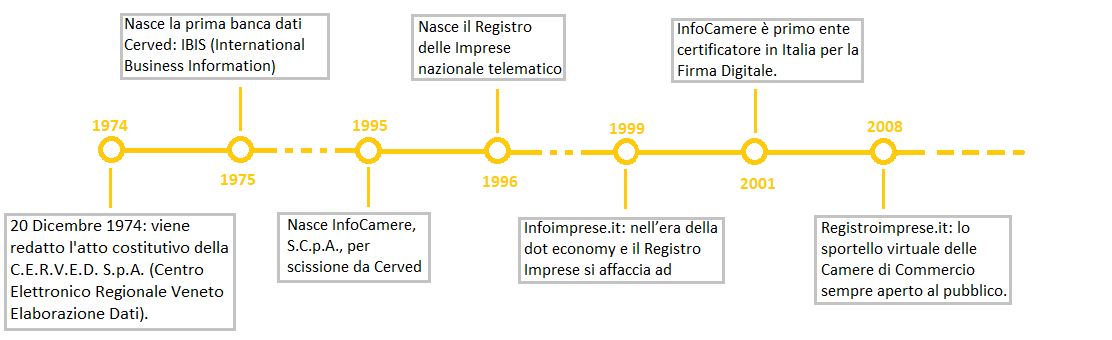
\includegraphics[width=13cm]{storyLine}
			\captionof{figure}{Storyline InfoCamere}
		\end{center}
	\end{figure}
	
	Le prime tecnologie informatiche aprivano nuovi orizzonti al trattamento massivo e veloce dei dati. Evolveva rapidamente la concezione di una gestione intelligente delle notizie amministrative sulla vita delle imprese, per trasformarle in informazioni rielaborabili ed utilizzabili in modi nuovi da tutti. Nasceva l’idea di valorizzare i dati ufficiali forniti dalle imprese, restituendoli al mercato e alle imprese stesse come informazioni utili per accrescere la propria competitività e progettare il proprio sviluppo.\\
	Si gettava il seme dell’efficienza nell’organizzazione delle Camere di Commercio, una base nuova per costruire un patto trasparente e vantaggioso tra imprese e Pubblica Amministrazione.
	
	\subsection{Anni '90: InfoCamere}
	All'inizio degli anni '90 aumentava sempre più la competizione globale e le sfide per portare l'Italia nella modernità. A tal fine, nel 1993, venne emanata una riforma (legge 29 Dicembre 1993, n. 580) che attribuiva alle Camere un'autonomia rispetto al governo centrale, mediante attribuzione della potestà statutaria e di autonomia finanziaria, oltre al riconoscimento del ruolo finalizzato alla pubblicizzazione delle imprese. Le Camere di Commercio Italiane hanno così modo di vedere un profondo rinnovamento in vari ambiti e, in particolar modo, nell'ambito tecnologico.
	
	\begin{figure}[htbp]
		\begin{center}
			
\includegraphics[height=3cm]{logo-infocamere}
			\captionof{figure}{Logo infocamere}
		\end{center}
	\end{figure}
	
	Nel 1995, per scissione da Cerved, nasce InfoCamere che raccoglie la sfida di realizzare il Registro delle imprese. Previsto dal codice civile fin dal 1942 e mai attuato, in due anni, con uno di anticipo sulle previsioni, il risultato è raggiunto: prende vita il primo esempio in Europa di registro pubblico sulle imprese  totalmente telematico; assieme ad un ecosistema di servizi sviluppati attorno al Registro delle imprese, è stato possibile semplificare i processi tra le imprese stesse e la Pubblica Amministrazione.
	
	\begin{figure}[htbp]
		\begin{center}
			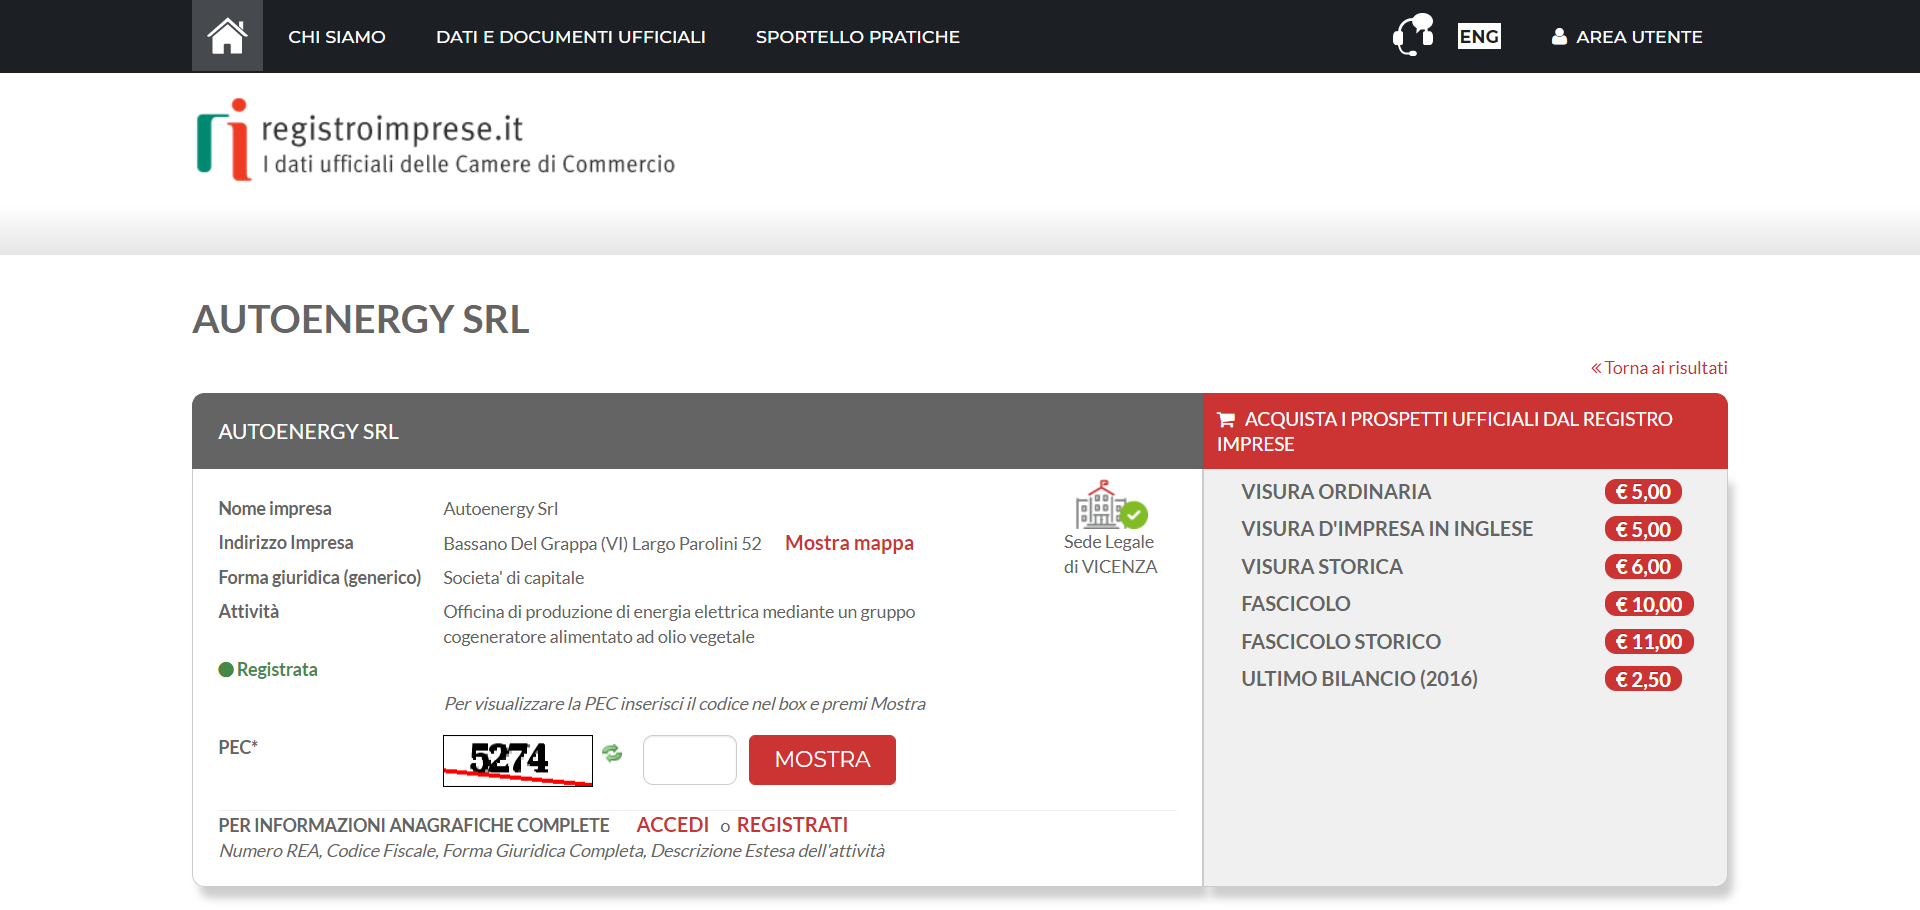
\includegraphics[width=13cm]{registro_imprese}
			\captionof{figure}{\cite{site:registro_imprese}}
		\end{center}
	\end{figure}
	
	A quella sfida ne seguono altre che rispondono ai nomi di ‘firma digitale’, ‘posta elettronica certificata’, ‘comunicazione unica’, ecc... . \\
	Attraverso InfoCamere, servizi e tecnologie digitali di frontiera diventavano patrimonio quotidiano della comunità delle imprese e dei professionisti, influendo sulle abitudini di lavoro di migliaia di italiani e stimolando i processi di innovazione nella Pubblica Amministrazione.

	\subsection{Servizi offerti}
	\nomeAzienda è la società consortile di informatica delle Camere di Commercio Italiane. Ha realizzato e gestisce il sistema telematico nazionale che collega tra loro tutte le Camere di Commercio, oltre alle rispettive sedi distaccate. 
	
	\begin{figure}[htbp]
		\begin{center}
			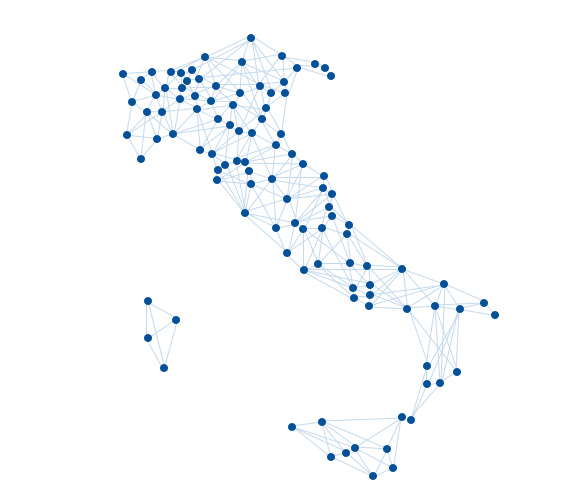
\includegraphics[height=8cm]{mappa_italia}
			\captionof{figure}{\cite{site:mappa_camere}}
		\end{center}
	\end{figure}
	
	Sua funzione istituzionale è anche la gestione e divulgazione del patrimonio informativo camerale, con particolare riferimento alle informazioni derivanti dal Registro delle imprese.\\
	Le banche dati camerali sono rese disponibili direttamente a imprese, pubbliche amministrazioni, professionisti e cittadini tramite il portale delle Camere di Commercio. \\
	La Società fornisce alle pubbliche amministrazioni l'accesso al Registro Imprese, assicurando loro l'accessibilità dei dati senza oneri, salvo quelli per la fornitura telematica e i servizi a valore aggiunto. \\
	Attraverso il sito del Registro delle imprese è possibile accedere agli strumenti per lo svolgimento delle pratiche telematiche, tra cui la Comunicazione Unica per l'attività d'impresa, valida anche per Agenzia delle Entrate, INPS, INAIL e Albo Artigiani. Il Registro Imprese è inoltre uno strumento di trasparenza amministrativa che fornisce un contributo importante nella lotta contro la criminalità economica. L'azienda ha infatti sviluppato per le autorità investigative alcuni servizi che, in questa direzione, consentono analisi mirate per monitorare fenomeni anomali. \\
	InfoCamere ha realizzato, per conto delle Camere di Commercio, l'infrastruttura tecnologica che garantisce il corretto funzionamento degli Sportelli Unici per le Attività Produttive (SUAP).
	
	\begin{figure}[htbp]
		\begin{center}
			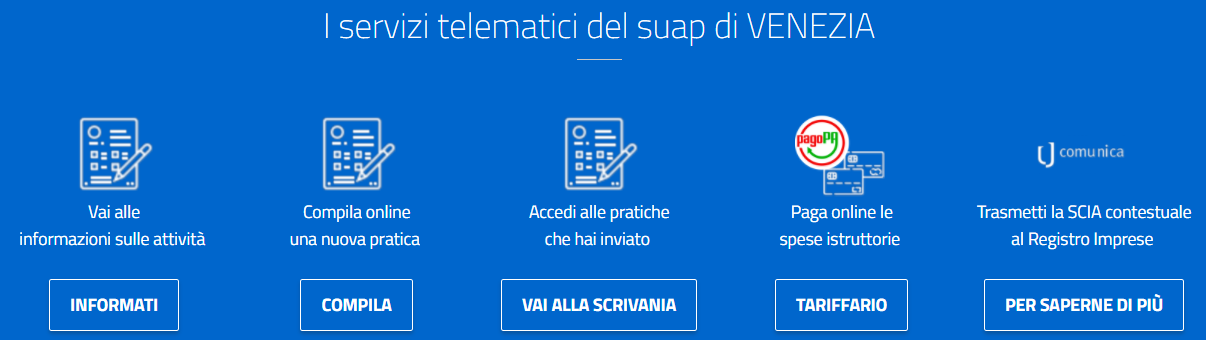
\includegraphics[height=4cm]{suap_venezia}
			\captionof{figure}{\cite{site:suap_venezia}}
		\end{center}
	\end{figure}
	
	Tra le realizzazioni di InfoCamere per il sistema camerale vi è anche la procedura informatica che consente di gestire il servizio di conciliazione online (Concilia Camera), fornendo così ad imprese, consumatori e professionisti uno strumento che permetta di ricevere assistenza specializzata nel raggiungimento di un accordo per risolvere in modo semplice, rapido, economico e sicuro una controversia, evitando di ricorrere alla giustizia ordinaria. \\
	InfoCamere è inoltre l'Autorità di Certificazione Nazionale che rilascia i certificati digitali delle Carte Tachigrafiche. \\
	La società si è infine dotata di un Sistema di Gestione della Sicurezza delle Informazioni certificato secondo lo standard ISO/IEC 27001, avendo conseguito nel 2012 la prima certificazione di conformità ISO/IEC 27001:2005 e a Marzo 2015 la ricertificazione secondo la nuova versione ISO/IEC 27001: 2013.

\section{Organizzazione aziendale}
\label{sec:organizzazione_aziendale}

	\begin{figure}[htbp]
		\begin{center}
			\includegraphics[width=12cm]{organigramma}
			\captionof{figure}{Organigramma aziendale}
		\end{center}
	\end{figure}

	In \nomeAzienda è possibile individuare 4 aree direzionali di maggior interesse:
	\begin{itemize}
		\item{Servizi alle Camere di Commercio;}
		\item{Servizi a imprese, Pubblica Amministrazione, professionisti e altri utenti;}
		\item{Tecnologie e impianti;}
		\item{Governo progetti, innovazione ed azienda digitale.}
	\end{itemize}

	Nello specifico, durante lo stage, ho preso parte all'area direzionale "Servizi alle Camere di Commercio". In quest'ultima è possibile individuare:
	\begin{itemize}
		\item{Area commerciale: si occupa degli accordi commerciali con le Camere di Commercio;}
		\item{Sviluppo ed erogazione servizi alle Camere: attua quanto accordato dall'area commerciale.}
	\end{itemize}

	In particolare, sono stato assegnato all'unità organizzativa denominata "Camera Digitale", che risponde allo "Sviluppo ed erogazione servizi alle Camere". Questa unità organizzativa si occupa delle digitalizzazione delle Camere, sia per quanto riguarda la gestione documentale, rispettando le norme riguardanti la conservazione dei documenti, sia per quanto riguarda i siti web informativi delle Camere di Commercio.

\section{Processi aziendali}
\label{sec:processi_aziendali}
In questa sezione presenterò i processi aziendali che principalmente coinvolgono l'unità organizzativa "Camera Digitale", con la quale ho avuto modo di confrontarmi.

	\subsection{La fornitura}
	L'azienda mette a disposizione dei clienti due differenti tipologie di prodotto e, nello specifico, di siti web:
	\begin{itemize}
		\item{\textbf{Listino}: rappresentano prodotti la cui forma, contenuto e funzione siano idonei alla replicazione;}
		\item{\textbf{Commessa}: rappresentano prodotti la cui forma, contenuto e funzione vengono fissate dal cliente.}
	\end{itemize}
	La contrattazione con il cliente viene interamente gestita dall'area commerciale. \\
	Se la tipologia di prodotto scelta dal cliente è di tipo "Commessa", si opera una raccolta dei requisiti a cui segue una proposta commerciale al cliente. \\
	In entrambe le tipologie di prodotto, quando l'offerta è stata concordata, la Camera di Commercio si occuperà dell'approvazione mediante una delibera pubblica. \\
	Una volta avvenuto l'ingaggio, se il prodotto appartiene alla tipologia "Listino", verrà assegnato al nuovo prodotto un codice identificativo generico; in caso contrario, se la tipologia è "Commessa", al prodotto sarà invece attribuito un codice specifico. \\
	A seguito dell'assegnazione di un nuovo codice identificativo del prodotto da realizzare, è possibile iniziare a sviluppare il sito web.
	
	\subsection{Ciclo di vita dei siti web}
	
	Il ciclo di vita dei siti web prodotti da InfoCamere, è così formato: 
	\begin{itemize}
		\item {\textbf{Sviluppo}: avviene lo sviluppo dei siti web e delle relative funzionalità; comprende specifici file system e database dedicati allo sviluppo, contenenti dati fittizi, oltre al software che dovrà essere, una volta pronto, distribuito;}
		\item {\textbf{Test}: segue lo sviluppo, dal quale prende in input il software prodotto. Il database è una copia del database di produzione del giorno precedente a quello considerato;}
		\item{\textbf{Produzione}: contiene il software che ha superato i test, e il database è popolato con dati inseriti direttamente dalla Camera di Commercio.}
	\end{itemize}

	\begin{figure}[htbp]
		\begin{center}
			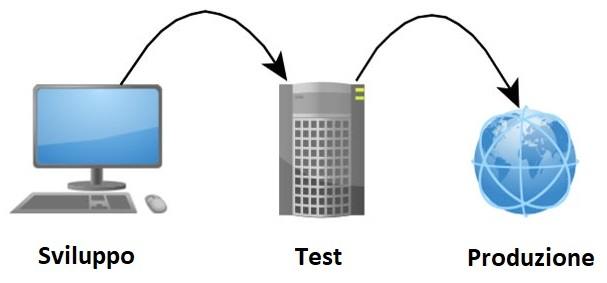
\includegraphics[height=5cm]{ciclo_di_vita}
			\captionof{figure}{Ciclo di vita dei siti web}
		\end{center}
	\end{figure}
	
	\subsection{Auditing}
	A seguito del caricamento dei contenuti da parte della Camera, nel sito sviluppato, parteciperanno al collaudo: il commerciale di InfoCamere che ha seguito il lavoro, un referente tecnico di InfoCamere e infine un referente tecnico della Camera di Commercio. Il prodotto di questo processo sarà un verbale del collaudo che dovrà essere firmato e protocollato, oltre a presentare la firma dei due referenti tecnici.
	
	\begin{figure}[htbp]
		\begin{center}
			
\includegraphics[height=2cm]{contratto}
			\captionof{figure}{Verbale firmato da entrambi i referenti tecnici}
		\end{center}
	\end{figure}

	\subsection{Manutenzione}
	Alla protocollazione del verbale prodotto dal collaudo, si può considerare concluso lo sviluppo del sito e prende avvio l'assistenza al prodotto.
		\subsubsection{Tipologie di manutenzione}
			La manutenzione può essere di 3 differenti tipologie:
			\begin{itemize}
				\item{\textbf{Correttiva}: vengono corretti bug presenti nel prodotto;}
				\item{\textbf{Adattativa}: i siti vengono adeguati a nuove norme in vigore;}
				\item{\textbf{Evolutiva}: vengono aggiunte funzionalità al sito; il prodotto subisce un'evoluzione: la natura del prodotto cambia in modo radicale, mantenendo però il prodotto stesso.}
			\end{itemize}

		\subsubsection{Gestione dei ticket}
		L'assistenza al prodotto viene gestita a più livelli, a cui affluiscono più gruppi di lavoro. \\
		Un nuovo ticket, prodotto di una segnalazione di un cliente, può essere gestito in modo autonomo dal primo livello o può essere assegnato ad un gruppo di lavoro appartenente al livello successivo. \\
		Il gruppo di lavoro a cui viene assegnato il nuovo ticket può:
		\begin{itemize}
			\item[--] {decidere di rifiutare il ticket: in questo caso, il ticket dovrà essere assegnato ad un altro gruppo di lavoro del secondo livello;}
			\item[--] {rimandare ad un altro gruppo di lavoro il ticket, nel caso in cui il gruppo identificato sia ritenuto più adatto a risolvere il problema;}
			\item[--] {decidere di utilizzare le proprie competenze per analizzare e cercare di risolvere il problema, fornendo eventualmente una soluzione e un tempo atteso.}
		\end{itemize}
	
		I ticket che richiedono una manutenzione evolutiva, comporteranno inoltre uno studio di fattibilità, fatto dal gruppo del secondo livello al quale il ticket è stato assegnato, e un successivo preventivo orario ed economico. \\
		Per i siti web, è garantito ai clienti un pacchetto di ore di supporto specificatamente per i ticket di tipo implementativo. Se il numero di ore preventivato è compreso nelle ore residue del pacchetto garantite al cliente, l'implementazione delle nuove funzionalità può avere luogo. In caso contrario, è necessaria la figura del commerciale per gestire la richiesta di manutenzione evolutiva.

\section{Tecnologie utilizzate}
\label{sec:tecnologie_utilizzate}
Di seguito, presenterò le tecnologie con cui sono venuto a contatto durante lo stage.
	
	\subsection{Ambiente di sviluppo}
	
		\subsubsection{Drupal}
		L'unità organizzativa alla quale ho preso parte, "Camera Digitale", realizzava i siti web con \gls{Drupal}. Si tratta di un \gls{CMSg}, rilasciato sotto licenza \gls{open source}, che permette la creazione di siti Internet, blog e portali, gallerie di immagini, forum di discussione, piattaforme intranet e molto altro. Essa è altresì un’applicazione completamente web based e può quindi essere utilizzata attraverso un semplice browser. \\
		E' interamente sviluppato in \gls{PHP} e utilizza come base di dati \gls{MySQL} in modo nativo.
		
		\begin{figure}[htbp]
			\begin{center}
				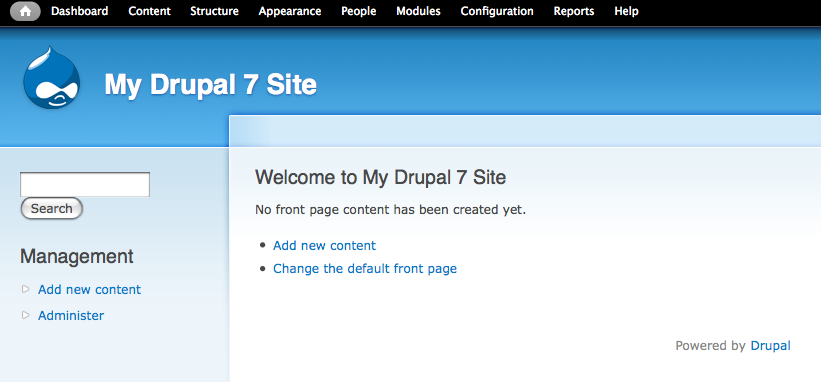
\includegraphics[height=4cm]{drupal}
				\captionof{figure}{\cite{site:drupal}}
			\end{center}
		\end{figure}
	
		\subsubsection{Acquia Dev Desktop 2}
		E’ un software che permette di realizzare e gestire siti dinamici, che possono accrescere e mutare il proprio contenuto continuamente.
		Di seguito, sono elencati i più importanti concetti chiave di questa tecnologia:
		\begin{itemize}
			\item {Gratuito per uso personale;}
			\item {E' il modo più veloce per disporre di un sistema \gls{Drupal}, fornendo un \gls{DAMPg} stack installer in modo tale da consentire l'installazione di tutte le componenti necessarie per avviare \gls{Drupal}, comprendente \gls{Apache}, \gls{MySQL} e \gls{PHP};}
			\item {Permette la gestione di più istanze \gls{Drupal} in modo semplice e veloce. Questa caratteristica risulta essere particolarmente significativa, in quanto ad ogni diversa tecnologia utilizzata per la ricerca è possibile associare una nuova istanza \gls{Drupal}, così da evitare interferenze tra le tecnologie e mantenere il lavoro ben distinto.}
		\end{itemize}
	
		\begin{figure}[htbp]
			\begin{center}
				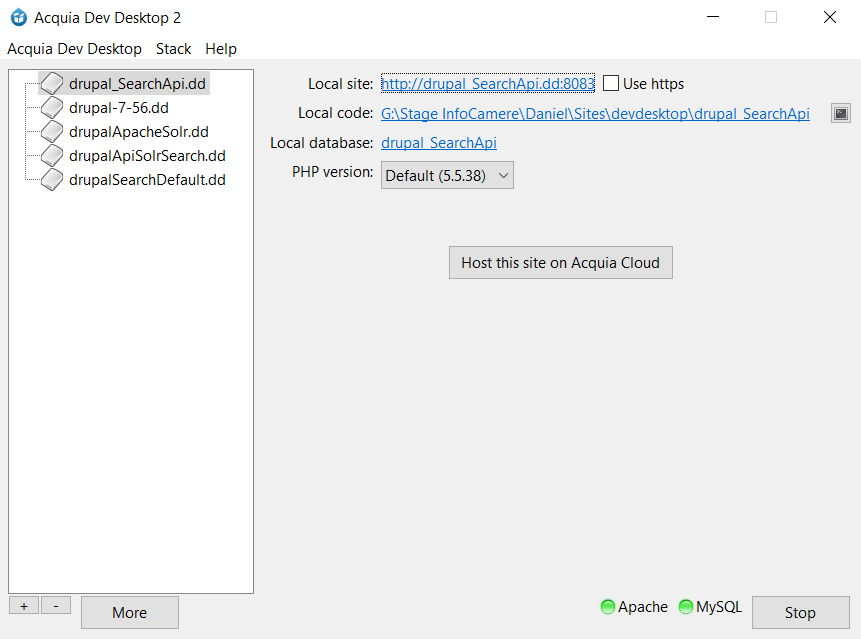
\includegraphics[width=9cm]{acquia}
				\captionof{figure}{Pannello di controllo di Acquia Dev Desktop 2}
			\end{center}
		\end{figure}
	
	\subsection{Gestione di versione}
	\gls{Git} è un sistema di controllo di versione distribuito e \gls{open source} ed è lo strumento utilizzato dall'azienda per il versionamento del codice. In particolare, viene utilizzato \gls{Git Extensions}, che rappresenta un'interfaccia grafica per \gls{Git}, permettendone l'utilizzo senza dover ricorrere alla riga di comando.
	Il materiale prodotto durante lo stage, comprensivo di copie delle istanze \gls{Drupal} create, è stato versionato. In questo modo è possibile prevenire eventuali perdite di dati derivanti dal malfunzionamento della macchina utilizzata, oltre a mantenere le varie versioni di quanto prodotto; in qualunque momento è dunque possibile ricreare l'ambiente di sviluppo di qualsiasi versione e recuperare tutti i prodotti realizzati.
		
	\subsection{Comunicazioni}
	\gls{Zimbra} è il client di posta elettronica utilizzato da \nomeAzienda. Questa tecnologia è \gls{open source} e prevede un sistema di chiamate vocali e messaggistica istantanea. La suite di comunicazione può essere configurata in base alle esigenze personali di ciascuna azienda. Con un servizio cloud installato su server dedicati, tutti gli strumenti di comunicazione aziendale sono facilmente gestibili e ottimizzabili. \\
	E' molto utile in ambito aziendale, per il coordinamento e la collaborazione tra colleghi.
	
	\begin{figure}[htbp]
		\begin{center}
			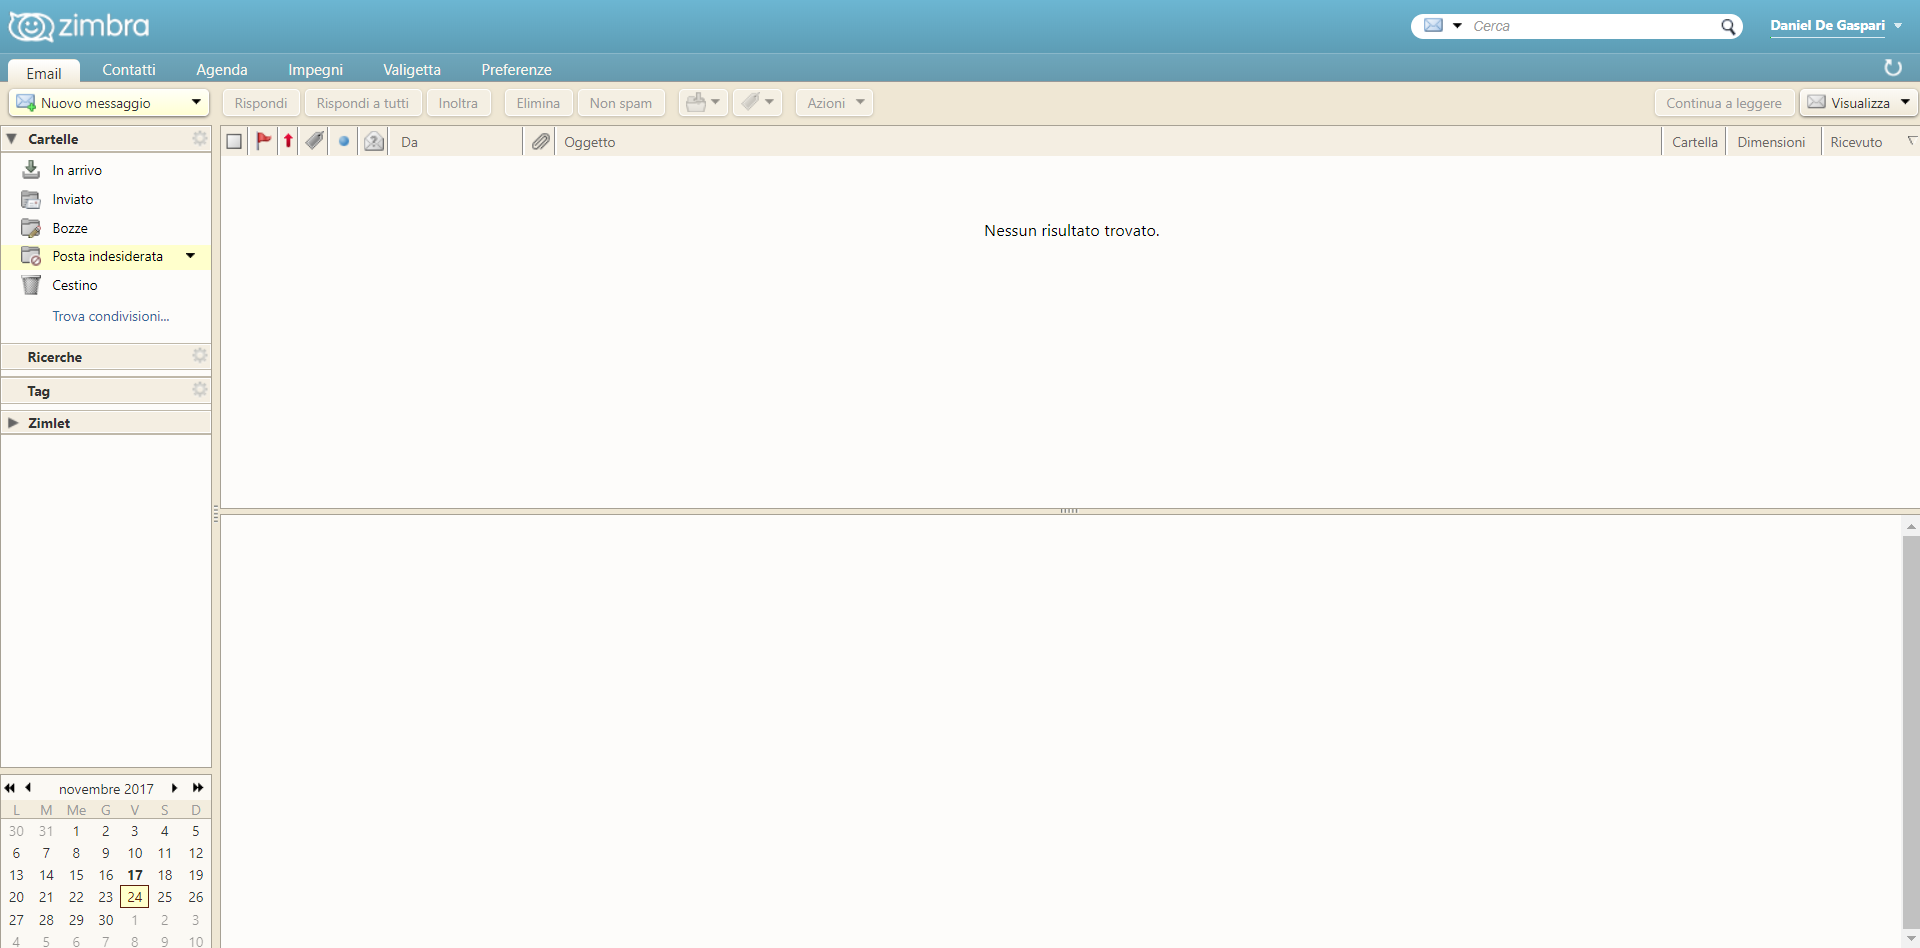
\includegraphics[height=6cm]{zimbra}
			\captionof{figure}{Client di posta elettronica Zimbra}
		\end{center}
	\end{figure}

\section{Rapporto con l'innovazione}
\label{sec:rapporto_con_innovazione}
\nomeAzienda guarda all'innovazione con grande interesse, tanto da avere un'area direzionale che tratta la materia dell'innovazione, come si può vedere nella sezione dedicata all'\hyperref[sec:organizzazione_aziendale]{organizzazione aziendale}. \\
Le Camere di Commercio demandano ad InfoCamere il compito di portare innovazione nei servizi che le stesse mettono a disposizione delle imprese, soprattutto nel loro rapporto con la Pubblica Amministrazione, con l'obietto di semplificare e alleggerire i costi burocratici e gestionali. In linea con questo principio, InfoCamere persegue la strada della dematerializzazione, della firma digitale, della conservazione sostitutiva della carta, della fatturazione elettronica e di tutti gli strumenti che la tecnologia e l'informatica offrono per garantire una governance delle procedure amministrative al passo con le esigenze delle imprese e coi tempi. \\
In quest'ottica rientrano tutti i servizi amministrativi che InfoCamere ha progettato nel tempo per conto delle Camere di Commercio Italiane: dall'invio online delle pratiche, allo Sportello Unico per le Attività Produttive, agli strumenti per le imprese dedicati alla giustizia civile, alla fatturazione elettronica, ai pagamenti verso le Pubbliche Amministrazioni fino a quelli di certificazione digitale, elemento essenziale per il funzionamento dei servizi online.
